\label{sect:simulation}
In order to experiment with robotic systems, a researcher requires a controllable robotic platform, a control system that interfaces to the robotic system and provides behaviors for the robot to carry out, and an environment to operate in. Our kitting application relies on an open source (the game engine is free, but license restrictions do apply), freely available framework capable of fulfilling all of these requirements. This framework is the Unified System for Automation and Robot Simulation (USARSim) \cite{USARSimWeb}. It provides the robotic platform and environment.

\subsection{The USARSim Framework}

USARSim~\cite{CARPIN.LNAI.2006,WANG.WSC.2003} is a high-fidelity physics-based simulation system based on the Unreal Developers Kit (UDK)~\cite{UDKWeb} from Epic Games. USARSim was originally developed under a National Science Foundation grant to study Robot, Agent, Person Teams in Urban Search and Rescue~\cite{LEWIS.ICHC.2003}. Since that time, it has been turned into a National Institute of Standards and Technology (NIST)-led, community-supported open source project that provides validated models of robots, sensors, and environments. Altogether, the Karma Physics engine~\cite{KarmEngine} and high-quality 3D rendering facilities of the Unreal game engine allow the creation of realistic simulation environments that provide the embodiment of a robotic system. Furthermore, USARSim comes with tools to develop objects and environments and it is possible to control the objects in the game through a Transmission Control Protocol/Internet Protocol (TCP/IP) socket with a host computer.

Through its usage of UDK, USARSim utilizes the physX physics engine~\cite{physXWeb} and high-quality 3D rendering facilities to create a realistic robotic system simulation environment. The current release of USARSim consists of various model environments, models of commercial and experimental robots, and sensor models. High fidelity at low cost is made possible by building the simulation on top of a game engine. By delegating  simulation specific tasks to a high volume commercial platform (available for free to most users) which provides superior visual rendering and physical modeling, full user effort can be devoted to the robotics-specific tasks of modeling platforms, control systems, sensors, interface tools and environments. These tasks are in turn accelerated by the advanced editing and development tools integrated with the game engine. This leads to a virtuous spiral in which a wide range of platforms can be modeled with greater fidelity in a short period of time.

%USARSim was originally based upon simulated environments in the Urban Search and Rescue (USAR) domain. Realistic disaster scenarios as well
%as robot test methods were created (Figure 1(a)). Since then, USARSim has been used worldwide and more environments have been developed for different purposes. Other environments such as the NIST campus (Figure 1(b)) and factories (Figure 1(c)) have been used to test the performance of algorithms in different efforts [9–11]. The simulation is also widely used for the RoboCup Virtual Robot Rescue Competition [12], the IEEE Virtual Manufacturing and Automation Challenge [13], and has been applied to the DARPsA Urban Challenge (Figure 1(d)).


%\begin{figure}[t!]
%\centering
%\subfigure[Test Room.]{\label{TestRoom}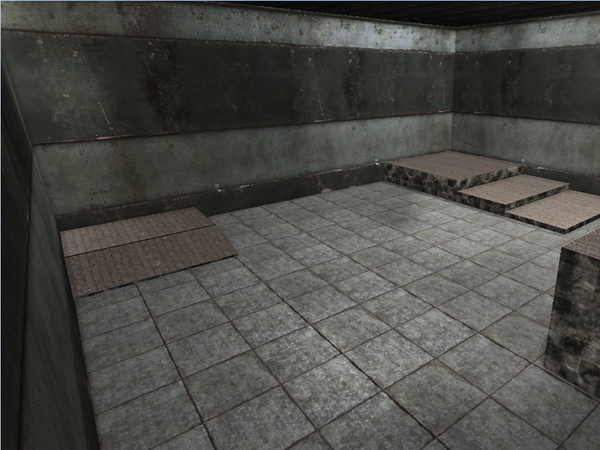
\includegraphics[width=4cm]{images/Worlds/testRoom.jpg}}\qquad
%\subfigure[Factory,]{\label{3D_World-c}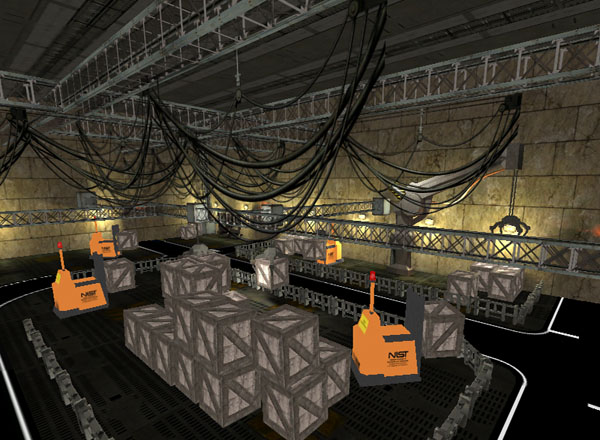
\includegraphics[width=4cm]{images/Worlds/factory.jpg}}
%\caption{Sample of 3D environments in USARSim.} \label{3D_World}
%\end{figure}
%\begin{figure}[t!]
%\centering
%\subfigure[Air Robot AR100B.]{\label{Fig:AirRobot}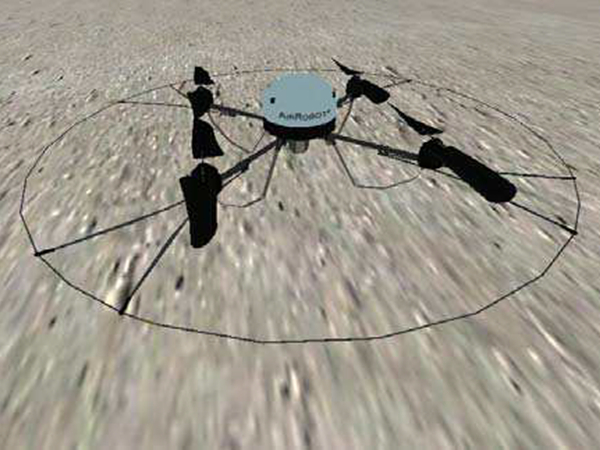
\includegraphics[width=4cm]{images/Robots/airRobot_2.jpg}}\qquad
%\subfigure[Kuka KR60,]{\label{Fig:KR60}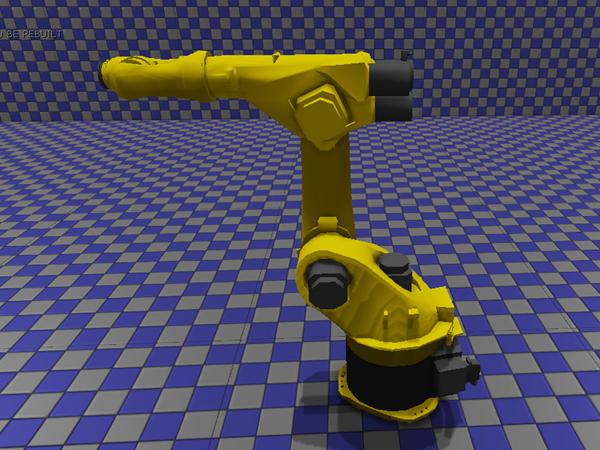
\includegraphics[width=4cm]{images/Robots/kr60.jpg}}
%\caption{Sample of vehicles in USARSim.}
%\end{figure}
%USARSim was initially developed with a focus on differential drive wheeled robots. However, USARSim's open source framework has encouraged wide community interest and support that now allows USARSim to offer multiple robots, including humanoid robots, aerial platforms (Figure~\ref{Fig:AirRobot}), robotic arms (Figure~\ref{Fig:KR60}), and commercial vehicles. All robots in USARSim have a chassis, and may contain multiple wheels, sensors, and
%actuators. The robots are configurable (e.g. specify types of
%sensors/end effectors) through a configuration file that is read at run-time. The properties of the robots can
%also be configured, such as the battery life and the frequency of
%data transmission.

%%--------------
USARSim was originally based upon simulated environments in the (Urban Search and Rescue) USAR domain. Realistic disaster scenarios as well as robot test methods were created (Figure~\ref{TestRoom}).
Since then, USARSim has been used worldwide and more environments have been developed for different purposes. Other environments such as the NIST campus (Figure~\ref{3D_World-b}) and factories (Figure~\ref{3D_World-c}) have been used to test the performance of algorithms in different efforts~\cite{WANG.HFES.2005,BALAGUER.IROS.2008,KOOTBALLY.ITEA.2010}. The simulation is also widely used for the RoboCup Virtual Robot Rescue Competition \cite{RoboCupWeb}, the IEEE Virtual Manufacturing and Automation Challenge \cite{VMACWeb}, and has been applied to the DARPA Urban Challenge (Figure~\ref{3D_World-a}).

\begin{figure}[t!]
\centering
\subfigure[Test Room.]{\label{TestRoom}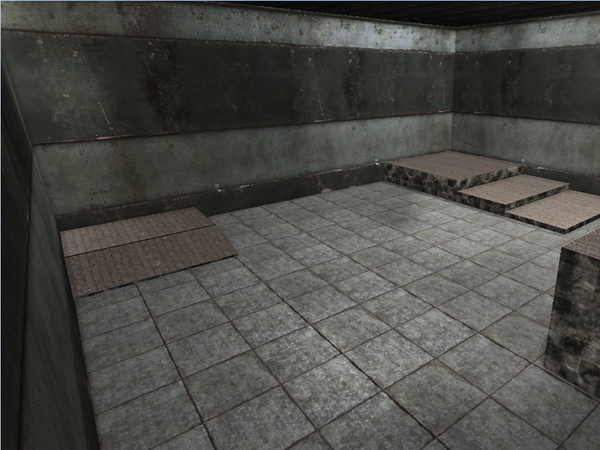
\includegraphics[width=4cm]{images/Worlds/testRoom.jpg}}\qquad
\subfigure[NIST main campus.]{\label{3D_World-b}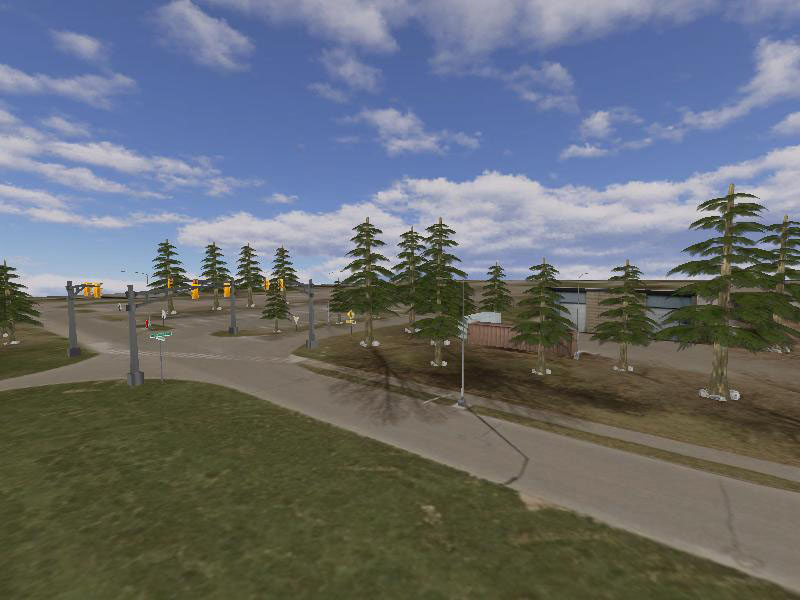
\includegraphics[width=4cm]{images/Worlds/nist2.jpg}}\qquad
\subfigure[Factory,]{\label{3D_World-c}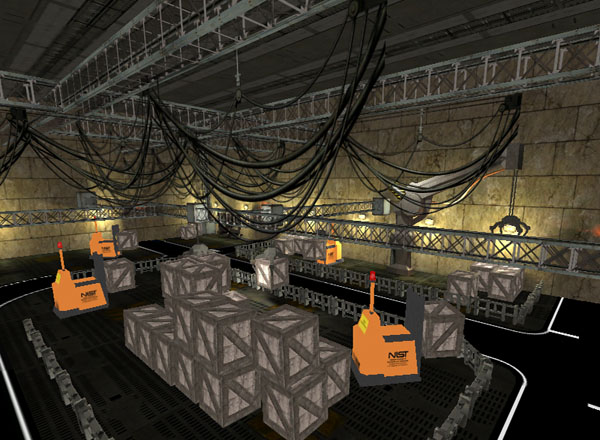
\includegraphics[width=4cm]{images/Worlds/factory.jpg}}\qquad%
\subfigure[Road course.]{\label{3D_World-a}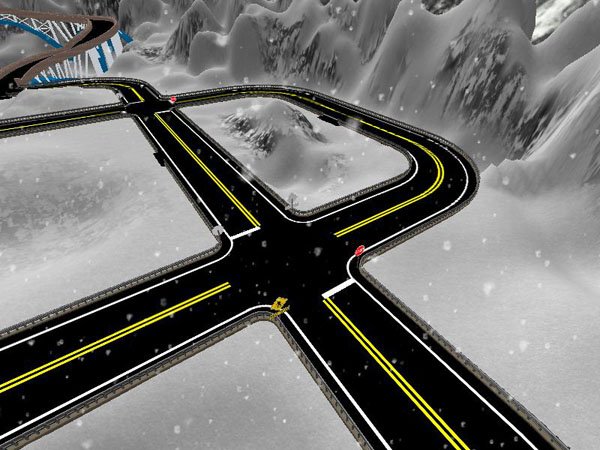
\includegraphics[width=4cm]{images/Worlds/arda1.jpg}}
\caption{Sample of 3D environments in USARSim.} \label{3D_World}
\end{figure}

USARSim was initially developed with a focus on differential drive wheeled robots. However, USARSim's open source framework has encouraged wide community interest and support that now allows USARSim to offer multiple robots, including humanoid robots (Figure~\ref{Fig:Nao}), aerial platforms (Figure~\ref{Fig:AirRobot}), robotic arms (Figure~\ref{Fig:KR60}), and commercial vehicles (Figure~\ref{Fig:Kiva}). In USARSim, robots are based on physical computer aided design (CAD) models of the real
robots and are implemented by specialization of specific existing classes. This structure allows for easier development of new platforms that model custom designs.

All robots in USARSim have a chassis, and may contain multiple wheels, sensors, and
actuators. The robots are configurable (e.g. specify types of
sensors/end effectors) through a configuration file that is read at run-time. The properties of the robots can
also be configured, such as the battery life and the frequency of
data transmission.

\begin{figure}[t!]
\centering
\subfigure[Aldebaran Robotics Nao.]{\label{Fig:Nao}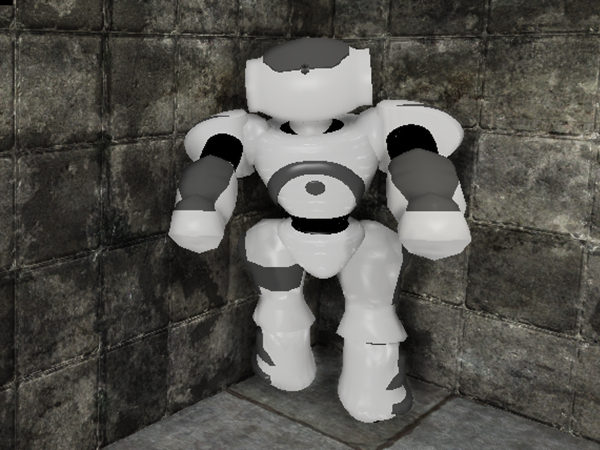
\includegraphics[width=4cm]{images/Robots/nao.jpg}}\qquad
\subfigure[Air Robot AR100B.]{\label{Fig:AirRobot}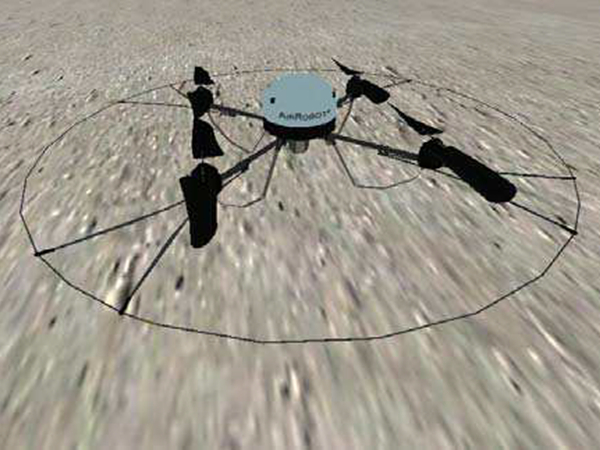
\includegraphics[width=4cm]{images/Robots/airRobot_2.jpg}}\qquad
\subfigure[Kuka KR60,]{\label{Fig:KR60}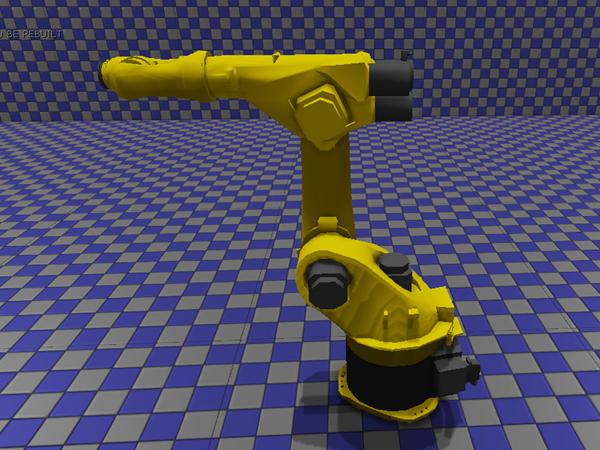
\includegraphics[width=4cm]{images/Robots/kr60.jpg}}\qquad
\subfigure[Kiva Robot.]{\label{Fig:Kiva}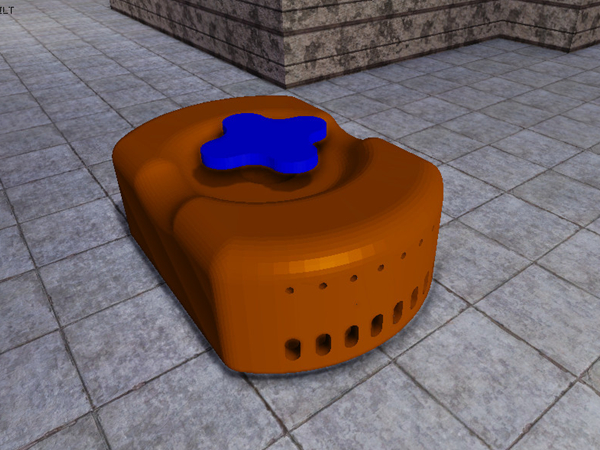
\includegraphics[width=4cm]{images/Robots/kiva.jpg}}
\caption{Sample of vehicles in USARSim.}
\end{figure}

\subsection{The Simulated Sensor System}
\label{subsection:usartruth}
Poses of objects in the virtual environment are retrieved with the USARTruth tool. USARTruth is capable of reading out information on objects in USARSim by connecting as a client to TCP socket port 3989. The simulator USARTruthConnection object listens for incoming connections on port 3989 and receives queries over a socket in the form of strings formatted into key-value pairs.

The USARTruth connection accepts two different keys, ``class'' and ``name''. When USARSim receives a new string over the connection, it sends a sequence of key-value formatted strings back over the socket, one for each Unreal Engine Actor object that matches the requested class and object names. An example of the strings returned by USARSim is given below along with a description for each key.


\{Name P3AT\_0\} \{Class P3AT\} \{Time 29.97\} \{Location 0.67,2.30,1.86\} \\ \{Rotation 0.00,0.46,0.00\} where:
%\{Name P3AT\_0\} \{Class P3AT\} \{Time 29.97\} \{Location 0.67,2.30,1.86\} \{Rotation 0.00,0.46,0.00\} where:
%The return strings include the following keys:

\begin{itemize}
\item Name: The internal name of the object in USARSim.
\item Class: The name of the most specific Unreal Engine class the object belongs to.
\item Time: The number of seconds that have elapsed since the simulator start, as a floating-point value.
\item Location: The comma-separated position of the object in global coordinates.
\item Rotation: The comma-separated orientation of the object in global coordinates, in roll, pitch, yaw form.
\end{itemize}


%The virtual sensor system uses USARTruth to simulate real-world sensors by opening a new USARTruth connection and sending one request for specified Unreal Engine class names.

% each different Unreal Engine class name found in the \textsf{MySQL Database}. For simulation purposes, the Unreal Engine class name is stored as an object's ``external shape''. It is important to note that the Location and Rotation values coming out of USARTruth do not include noises and assume perfect sensor data.
%
% The system then parses the data coming in from USARTruth and updates the relative pose in the MySQL database for each object returned. Since USARTruth returns object locations in global coordinates, the relative pose for each object is updated without changing its transformation tree; that is, the RefObject for its PhysicalLocation is unchanged. The actual updated relative pose is computed according to
% \begin{equation}
% L' = LG^{-1}G'
% \end{equation}
% where $L'$ is the updated relative transformation, $L$ is the old relative transformation (read from the MySQL database), $G$ is the old global transformation (computed from the transformation tree in the database), and $G'$ is the updated global transformation (retrieved from USARTruth).
